\IEEEraisesectionheading{\section{简介}
\label{sec:introduction}}

基于视频的运动目标检测是将视频序列图像中的变化区域从场景中分割出来,其中,视频序列图像中变化的区域被称为前景,而其他区域被称为背景。运动目标检测是对运动目标进行行为理解和分析的前提和基础,在智能监控、用户交互等领域有着广泛的应用前景。

传统的运动目标检测方法主要包括帧间差分法、背景差分法和光流法。其中,因受计算复杂、抗噪性能差且不利于实现等条件的制约,光流法一般不适用于视频序列图像中的运动目标检测。而基于差分的方法,帧间差分法比较容易收到运动目标的速度影响,无法对运动速度过快或过慢的目标进行较好的检测。而在检测较大面积的运动物体时,易出现目标“空洞”等问题,不利于下游任务。与帧间差分法相比,背景差分法获得的运动目标信息更完整,位置更准确,且实现简单。

背景差分法是通过判断当前帧和背景帧的对应像素点的变化程度来判断当前像素是否属于运动目标。如果对应的像素点变化值小于设定的阈值,则该像素背标记为背景像素,否则为前景像素。从理论上来看,只要能有合适的背景和适当的图像处理,运动目标就可以被较快且较为准确的检测并分割出来。

但在实际应用中,由于背景差分法对背景的依赖非常大。一个朴素的背景建模方法是对在一段时间内的图像进行平均,创建与当前静态场景相似的背景近似值。虽然这在对象连续移动并且背景在大部分时间可见的情况下是有效的,但是对于具有许多运动目标的场景,尤其是当它们移动缓慢时,这种背景建模方法是不鲁棒的。

从统计的角度看,图像中每个像素点的值在短时间内都是围绕某一中心值一定距离的分布。通常,中心值可以用均值来代替,距离则可以用方差来代替。如果数据点足够多的话,是可以说这些点呈高斯分布。由此,若像素点的值偏离均值较远(超出一定方差范围),那么该像素属于前景,否则认为该点属于背景。

\begin{figure}[!ht]
  \centering
  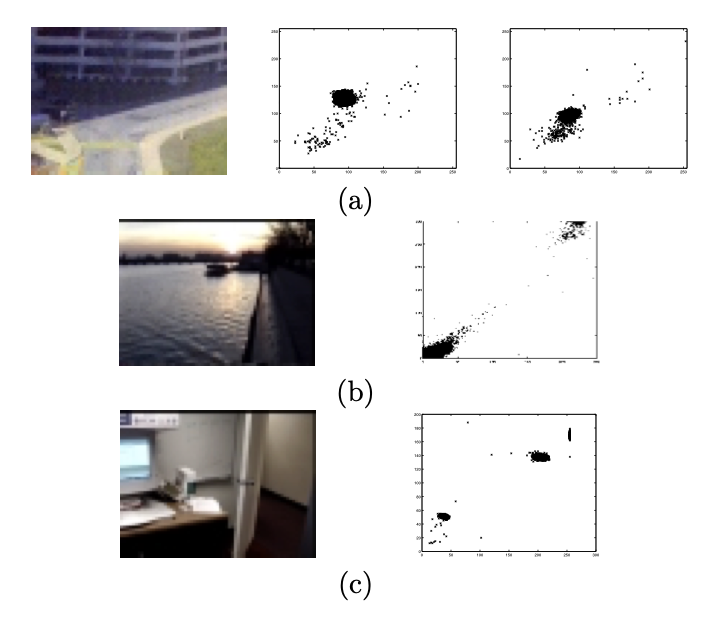
\includegraphics[width=\linewidth]{fig1.png}
  \caption{视频序列中某一帧图像和图像中单个像素的值随时间变化的散点图:(a)来自相同像素相隔2分钟的散点图;(b)由水面的镜面反射造成的像素值的两个分布;(c)监视器闪烁导致的像素值的两个分布.}
  \label{fig:light_change}
  \vspace{-0.5cm}
\end{figure}

但场景中光照的变化会给这种背景建模方法带来挑战。如图 \ref{fig:light_change} 所示,如果图像中的每个像素值都是在特定光照条件下的特定表面产生的,则在考虑图像采集噪声的同时,单个高斯模型将足以对该像素值建模描述。如果只是光照随时间变化,每个像素用单个自适应高斯建模也足够了。然而实际上,图像某一位置的像素值可能来自于多个表面(如树叶的抖动),并且光照条件也会发生改变。因此,单高斯模型只能描述背景的单一模式,当背景表现为树叶晃动或水面反射的光照变化等多模态形式时就容易出错。这就需要使用自适应高斯混合模型来对背景进行建模。

本文在视频帧序列实现基于高斯混合模型的背景建模,分别采用了手动实现和调用 OpenCV 的函数两种方式。本文剩余部分将对高斯混合模型的背景建模方法的原理、实现及实验进行介绍,所有实验涉及的方法、函数实现均基于 Python 语言。